\documentclass[tikz,border=2pt]{standalone}
\usepackage{tikz}
\usepackage[european]{circuitikz}
\usetikzlibrary{arrows.meta,positioning,calc}
../cictikz/src/cictikz/data/tex/cictikz_lib.tex
\begin{document}
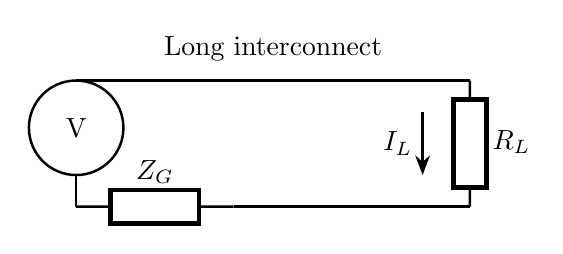
\begin{tikzpicture}[>=Stealth, line width=0.9pt]
  \draw (0,0) circle (0.6) node {V};
  \draw (0,-0.6) -- (0,-1.0);
  \draw (0,-1.0) to[R,l=$Z_G$] (2,-1.0);
  \draw (2,-1.0) -- (5,-1.0);
  \draw (0,0.6) -- (5,0.6);
  \draw (5,0.6) to[resistor,l=$R_L$] (5,-1.0);
  \draw[->] (4.4,0.2) -- (4.4,-0.6) node[midway,left] {$I_L$};
  \node at (2.5,1.0) {Long interconnect};
\end{tikzpicture}
\end{document}
